\documentclass{beamer}

\mode<presentation>
{
  \usetheme[minimal, numbers, totalnumbers]{Statmod}
}

\usepackage[russian]{babel}
\usepackage[utf8]{inputenc}
\usepackage{cancel}
\usepackage{graphicx}
\graphicspath{{pictures/}}
\DeclareGraphicsExtensions{.pdf,.png,.jpg}
\usepackage[T1]{fontenc}
\DeclareMathOperator*{\argmin}{arg\,min}

\title[Кластеризация и тематические модели]
{Обучение без учителя. Кластеризация. Тематическое моделирование}

\author[Гоголева, Капаца, Мандрикова]{Елена Гоголева, Дейвид Капаца, Анастасия Мандрикова}

\institute
{
  Санкт-Петербургский государственный университет\\
  Прикладная математика и информатика\\
  Вычислительная стохастика и статистические модели\\
  \vspace{0.5cm}
  Семинар по статистическому и машинному обучению\\
}

\date{Ноябрь 2021}


\begin{document}

\begin{frame}
  \titlepage
\end{frame}

\begin{frame}{План доклада}
\begin{enumerate}
    \item Обучение без учителя
    \begin{itemize}
        \item Типы задач и методы их решения
    \end{itemize}
    \item Кластеризация
    \begin{itemize}
        \item Постановка задачи
        \item Некорректность задачи
        \item Вероятностный подход
        \begin{itemize}
            \item EM-алгоритм для задачи разделения смеси распределений
            \item k-means и его связь с EM-алгоритмом
        \end{itemize}
        \item Иерархическая кластеризация
        \begin{itemize}
            \item Формула Ланса-Уильямса
            \item Визуализация кластерной структуры
        \end{itemize}
        \item Функционалы качества кластеризации
        \item Другие подходы и методы (FOREL, DBSCAN, карты Кохонена)
    \end{itemize}
\end{enumerate}
\end{frame}

\begin{frame}{План доклада (продолжение)}
\begin{enumerate}
\setcounter{enumi}{2}
    \item Тематические модели 
    \begin{itemize}
        \item Введение
        \item Вероятностная модель коллекции документов
        \begin{itemize}
            \item Постановка задачи
            \item Гипотезы
            \item Предварительная обработка документов
        \end{itemize}
        \item PLSA
        \begin{itemize}
            \item Стохастическое матричное разложение
            \item Принцип максимума правдоподобия
            \item EM-алгоритм
            \item Начальное приближение
        \end{itemize}
        \item Критерии качества модели
    \end{itemize}
\end{enumerate}
\end{frame}

%%%%%%%%%%%%%%%%%%%%%%%%%%%%%%%%%%%%%%%%%%%%%%%%%%%%%%%%%%%%%%%%%

\begin{frame}{Типы задач и методы их решения}
    В случае обучения с учителем известны как независимые переменные $X_{1}, ... , X_{p},$ так и зависимая переменная $Y$. В случае обучения без учителя известны лишь $X_{1}, ... , X_{p}$. 
    
    \begin{itemize}
    
    \item Задачи сокращения размерности (PCA)
    
    \item Задачи визуализации данных (иерархическая кластеризация)

    \item Задачи кластеризации (k-means)
    
    \end{itemize}
    \end{frame}

%%%%%%%%%%%%%%%%%%%%%%%%%%%%%%%%%%%%%%%%%%%%%%%%%%%%%%%%%%%%%%%%%

\begin{frame}{Постановка задачи}

\textbf{Дано}:

$X$ --- пространство объектов;

$X^{n}  = \{X_{i}\}_{i = 1}^{n} \subset X$ --- обучающая выборка;

$X_{i} \in \mathrm{R^{p}}$ --- объекты определяемые вектором признаков;

$\rho : X \times X \rightarrow [0,\infty).$

\textbf{Найти}:

$a: X \rightarrow C$, где $C$ --- множество непересекающихся кластеров, таких что в каждый кластер попадают близкие относительно выбранной метрики $\rho$ индивиды.

\end{frame}


\begin{frame}{Этапы кластеризации}
Общая схема кластеризации состоит из: 

\begin{itemize}
    
    \item выбор метрики
    
    \item разделение на кластеры
    
    \item оценка качества кластеризации
    
    \item выделение признаков которые значимы для кластеризации
    
    \item интерпретация результатов

    \end{itemize}
   
   
\end{frame}

%%%%%%%%%%%%%%%%%%%%%%%%%%%%%%%%%%%%%%%%%%%%%%%%%%%%%%%%%%%%%%%%%

\begin{frame}{Форма кластеров}

    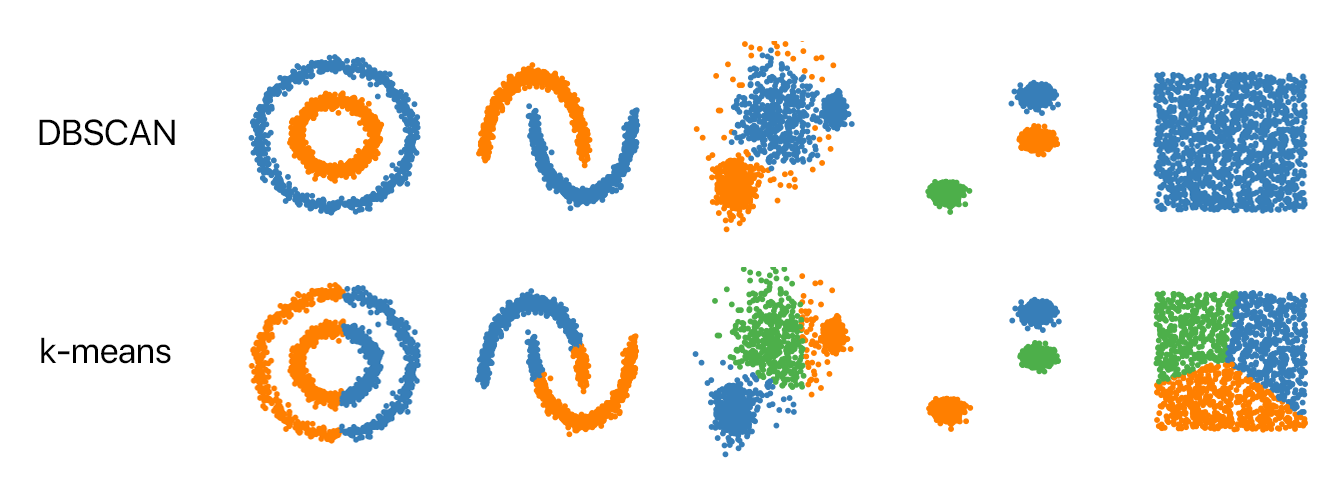
\includegraphics[scale = 0.25]{shape.png}
    
    \end{frame}



%%%%%%%%%%%%%%%%%%%%%%%%%%%%%%%%%%%%%%%%%%%%%%%%%%%%%%%%%%%%%%%%%

\begin{frame}{Некорректность задачи}

    \begin{itemize}
    
    \item Задача кластеризации не формализована
    
    \item Не всегда известно число кластеров
    
    \item Результат зависит от выбранной метрики $\rho$
    
    \item Разнообразие критериев качества
    
    \item Выбор метода кластеризации

    \end{itemize}
    
    \end{frame}


%%%%%%%%%%%%%%%%%%%%%%%%%%%%%%%%%%%%%%%%%%%%%%%%%%%%%%%%%%%%%%%%%%%%%

\begin{frame}{Вероятностный подход}

Пусть, модель данных состоит из смеси k распределений:

$$
p(x) = \sum\limits_{i=1}^k \omega_{i} p_{i}(x)
$$


Оценить по наблюдаемой выборке из $p(x)$:

\begin{itemize}
\item $\omega_{1}\ldots \omega_{k}$ --- априорные вероятности появления обьектов из соответствующих кластеров;

\item $p_{1}(x)\ldots p_{k}(x)$ --- плотности распределения признаков внутри кластеров.
\end{itemize}
\end{frame}

%%%%%%%%%%%%%%%%%%%%%%%%%%%%%%%%%%%%%%%%%%%%%%%%%%%%%%%%%%%%%%%%%

\begin{frame}{EM - алгоритм}


Предположим принадлежность $p_{1}(x)\ldots p_{k}(x)$ одному семейству распределений:

$$
p_{i}(x) = \varphi(\theta_{i}; x).
$$

Согласно методу максимального правдоподобия:

$$
\omega, \theta =  \underset{\omega, \theta}{\text{argmax}} \sum\limits_{i=1}^n \ln  \sum\limits_{j=1}^k \omega_{j} \varphi(\theta_{j}; x_{i}).
$$
\end{frame}

%%%%%%%%%%%%%%%%%%%%%%%%%%%%%%%%%%%%%%%%%%%%%%%%%%%%%%%%%%%%%%%%%


\begin{frame}{EM - алгоритм}

Скрытые переменные $h_{ij} = P(\theta_{j}|x_{i})$ --- это вероятность того, что индивид $x_{i}$ принадлежит $j$ смеси. Найдем по формуле Байеса:
$$
h_{ij} = \frac{ \omega_{j} \varphi(\theta_{j}; x_{i})}{\sum\limits_{s=1}^k \omega_{s} \varphi(\theta_{s}; x_{i})}.
$$

Для любого индивида $\sum\limits_{j=1}^k h_{ij} = 1.$

\end{frame}

%%%%%%%%%%%%%%%%%%%%%%%%%%%%%%%%%%%%%%%%%%%%%%%%%%%%%%%%%%%%%%%%%


\begin{frame}{EM - алгоритм}

\textbf{E - шаг:}

Подставляем текущую оценку $\omega, \theta$ и расчитываем скрытые переменные  $h_{ij}$.

\textbf{M - шаг:}

Решение методом Лагранжа для максимизации ($\sum\limits_{j=1}^k\omega_{j} = 1$) даёт оценку для параметров:
$$
\omega_{j} = \frac{1}{n} \sum\limits_{i=1}^n h_{ij},
$$
$$
\theta_{j} = \underset{\theta}{\text{argmax}} \sum\limits_{i=1}^n h_{ij} \ln{\varphi(x_{i}, \theta)}.
$$

\end{frame}

%%%%%%%%%%%%%%%%%%%%%%%%%%%%%%%%%%%%%%%%%%%%%%%%%%%%%%%%%%%%%%%%%

\begin{frame}{k-means}

В качестве меры близости выбрано евклидово расстояние: 
$$
d(x_{i}, x_{i'}) = \sum\limits_{j=1}^k (x_{ij} - x_{i'j})^{2} = \| x_{i} - x_{i'} \|^{2}.
$$
Минимизируем меру близости между индивидами внутри одного кластера:
$$
\underset{C_{1},\ldots, C_{k}}\min \left\{ \sum\limits_{l=1}^k \frac{1}{|C_{l}|} \sum\limits_{i,i' \in C_{l}}   \| x_{i} - x_{i'} \|^{2} \right\}.
$$

\end{frame}

%%%%%%%%%%%%%%%%%%%%%%%%%%%%%%%%%%%%%%%%%%%%%%%%%%%%%%%%%%%%%%%%%

\begin{frame}{k-means}
1. Выбираем $\mu_{1},\ldots, \mu_{k}$ -- центры кластеров случайным образом.

2. Определяем принадлежность индивидов кластерам. $$C(i) = \underset{0 \leq j \leq  k}{\text{argmin}} \|x_{i} - \mu_{j} \|^{2}.$$

3. Для каждого кластера $C_{j}$ пересчитываем центры $\mu_{j}$ как выборочное среднее индивидов, которые были отнесены к этому кластеру.

4. Повторяем шаги 2 и 3 пока принадлежность кластерам не перестанет изменяться.
\end{frame}


%%%%%%%%%%%%%%%%%%%%%%%%%%%%%%%%%%%%%%%%%%%%%%%%%%%%%%%%%%%%%%%%%

\begin{frame}{k-means и его связь с EM - алгоритмом}

Алгоритм k-средних является частным случаем для гауссовой смеси распределения с диагональными матрицами, у которых одинаковые значения на диагоналях. 

В таком случае:

1) На Е-шаге мы не считаем вероятности принадлежности кластерам, а приписываем каждый объект одному кластеру (вероятность принадлежности будет равна 0 или 1);

2) Форма кластеров не настраивается: они все являются сферическими.

\end{frame}

\begin{frame}{Алгоритм агломеративной иерархической кластеризации}
    \begin{enumerate}
        \item Одноэлементые кластеры:\\
        $C_1 = \left\{\{x_1\}, \dots, \{x_n\}\right\}; \; R_1 = 0$\\
        $\forall\, i \neq j \text{ вычислить } R(\{x_i\}, \{x_j\})$
        \item для всех $t = 2, \dots, n$ ($t$ --- номер итерации)
        \item найти в $C_{t-1}$ два ближайших кластера:\\
        $(U, V) = \argmin\limits_{U \neq V}R(U, V), \; R_t = R(U, V)$
        \item слить их в один кластер:\\
        $W = U \cup V; \; C_t = C_{t-1} \cup W \backslash \{U, V\}$
        \item для всех $S \in C_t \backslash W $
        \item вычислить R(W, S)
    \end{enumerate}
\end{frame}

\begin{frame}{Формула Ланса--Уильямса}
    Позволяет обобщить большинство способов определить расстояние между кластерами
    \begin{equation*}
        R(W, S),\; W = U \cup V,\, U,\, V,\, S \subset X,
    \end{equation*}
зная расстояния
\begin{equation*}
        R(U, S),\, R(V, S),\, R(U, V).
    \end{equation*}
\begin{equation*}
    R(W, S) = \alpha_{U}U R(U, S) + \alpha_{V} R(V, S) + \beta R(U, V) + \gamma|R(U, S) − R(V, S)|,\quad \alpha_{U}, \alpha_{V} , \beta, \gamma \in \mathrm{R}.
\end{equation*}
\vspace{2\ex}
Например,
\begin{itemize}
    \item Расстояние Уорда:
\begin{equation*}
R(W, S) = \frac{|S||W|}{|S|+|W|}\rho^{2}\left(\sum\limits_{w\in W}\frac{w}{|W|}, \sum\limits_{s\in S}\frac{s}{|S|}\right);
\end{equation*}
\begin{equation*}
\alpha_U = \frac{|S|+|U|}{|S|+|W|},\, \alpha_V = \frac{|S|+|V|}{|S|+|W|},\, \beta = -\frac{|S|}{|S|+|W|},\, \gamma = 0.
\end{equation*}
\end{itemize}
\end{frame}

\begin{frame}{Визуализация кластерной структуры}
   \begin{block}{Определение}
   Дендрограмма --- древовидный график расстояний, при которых произошло слияние кластеров на каждом шаге
   \end{block}
   \begin{figure}
   \vspace{-2ex}
   \begin{center}
   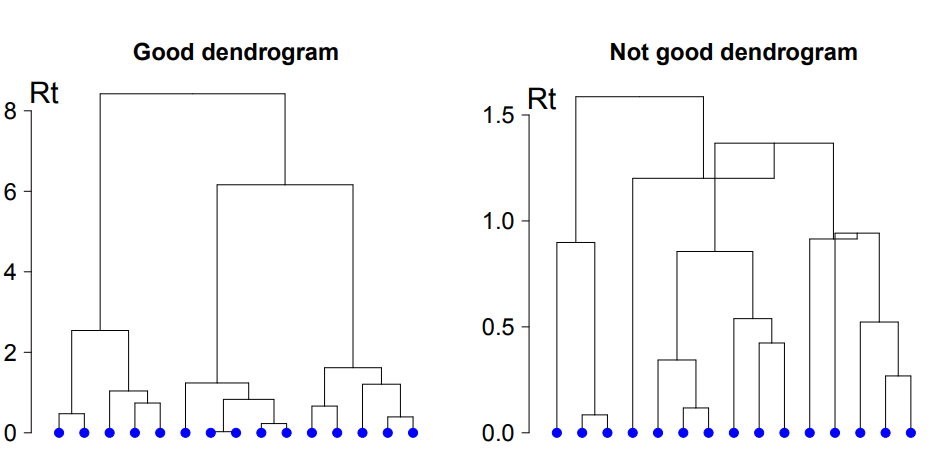
\includegraphics[scale = 0.4]{dendrogram.png}
   \end{center}
   \end{figure}
\end{frame}

\begin{frame}{Пример}
	\begin{figure}
	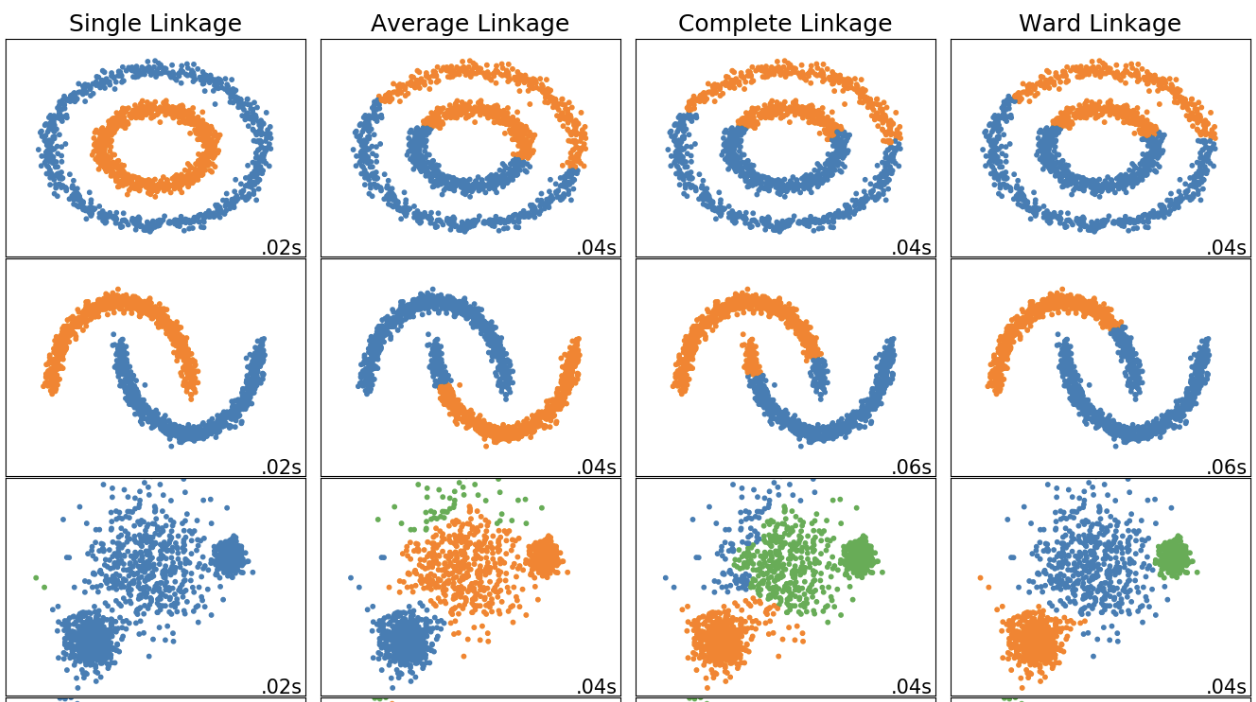
\includegraphics[scale = 0.25]{metrics.png}
	\end{figure}
\end{frame}

\begin{frame}{Другие алгоритмы кластеризации (FOREL)}
   FOREL (ФОРмальный ЭЛемент) --- алгоритм, основанный на идее объединения в один кластер объектов в областях их наибольшего сгущения.
   \vspace{2\ex}
   \begin{enumerate}
       \item Пусть $U = X_m$
       \item \textbf{Пока} есть некластеризованные точки, т.е. $U \neq \varnothing$;
       \item \quadвзять случайную точку $x_0 \in U$;
       \item \quad\textbf{Повторять}
       \item \quad\quadобразовать кластер с центром в $x_0$ и радиусом $R$:\\
       \quad\quad $K_0 = \{x_i \in U |\, \rho(x_i, x_0) \leq R\}$;
       \item \quad\quadпереместить центр $x_0$ в центр масс кластера:\\
       \quad\quad $x_0 = \frac{1}{|K_0|}\sum\limits_{x_i \in K_0}x_i$;
       \item \quad\textbf{Пока} состав кластера $K_0$ не стабилизируется;
       \item \quadПометить объекты внутри сферы как клаcтеризованные,\\ \quad $U = U \backslash K_0$.
   \end{enumerate}
\end{frame}

\begin{frame}{Преимущества и недостатки алгоритма FOREL}
   \textbf{Преимущества}\\
   \begin{itemize}
       \item Получаем двухуровневую систему кластеров;
       \item Кластеры могут быть произвольной формы\\ (при добавлении модификации к построению сферы);
       \item Варьируя $R$ можно управлять детальностью кластеризации.
   \end{itemize}
   \vspace{4\ex}
   \textbf{Недостатки}\\
   \begin{itemize}
       \item Алгоритм очень чувствителен к $R$ и к начальному выбору точки $x_0$
   \end{itemize}
\end{frame}

\begin{frame}{DBSCAN\\ \footnotesize(Density-based spatial clustering of applications with noise)}
   Объект $x \in U$, его $\epsilon$-окрестность $U_{\epsilon}(x) = \{u \in U: \rho(x, u) \leq \epsilon\}$ Каждый объект может быть одного из трёх типов:
   \begin{itemize}
       \item корневой: имеет плотную окрестность $|U_{\epsilon}(x)| > m$
       \item граничный: не корневой, но находится в окрестности корневого
       \item выброс: не корневой и не граничный.
   \end{itemize}
   \begin{figure}
   \vspace{-2\ex}
   \begin{center}
   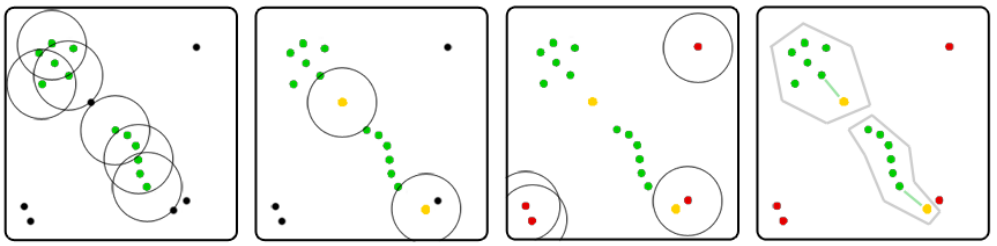
\includegraphics[scale = 0.4]{DBSCAN.png}
   \caption{\footnotesizeИллюстрация к алгоритму DBSCAN. На рисунке зелёным отмечены корневые объекты, жёлтым --- граничные и красным~---~шумовые.}
   \end{center}
   \end{figure}
\end{frame}

\begin{frame}{Алгоритм DBSCAN}
\textbf{Вход:} Выборка $X^{n} = \{x_1, \ldotsm x_{n}\}$, параметры $\epsilon$ и  $m$;\\
\textbf{Выход:} разбиение выборки на кластеры и шумовые выбросы;
    \begin{enumerate}
       \item $U = X_m,\; a = 0$;
       \item \textbf{Пока} есть некластеризованные точки, т.е. $U \neq \varnothing$;
       \item \quadвзять случайную точку $x \in U$;
       \item \quad\textbf{если} $|U_{\epsilon}(x)| < m$, \textbf{то}
       \item \quad\quad пометить $x$ как возможно шумовой;
       \item \quad\textbf{иначе}
       \item \quad\quad создать новый кластер: $K = U_{\epsilon}(x),\; a = a + 1$;
       \item \quad\quad\textbf{для всех} $x^{'} \in K$
       \item \quad\quad\quad\textbf{если} $|U_{\epsilon}(x^{'})| > m$ \textbf{то} $K = K \cup U_{\epsilon}(x^{'})$;
       \item \quad\quad\quad\textbf{иначе} пометить $x^{'}$ как граничный элемент $K$;
       \item \quad\quad$a_i = a$ для всех $x^{'} \in K$;
       \item \quad\quad$U = U\backslash K$.
   \end{enumerate}
\end{frame}

\begin{frame}{Преимущества и недостатки алгоритма DBSCAN}
   \textbf{Преимущества}\\
   \begin{itemize}
       \item Быстрая кластеризация больших данных (от $O(m \ln m)$ до $O(m^2)$ в зависимости от реализации);
       \item Кластеры произвольной формы;
       \item Явная разметка шумовых объектов;
   \end{itemize}
   \vspace{4\ex}
   \textbf{Недостатки}\\
   \begin{itemize}
       \item Алгоритм может неадекватно обрабатывать сильные вариации плотности данных внутри кластера, проёмы и шумовые мосты между кластерами.
   \end{itemize}
\end{frame}

\begin{frame}{Пример}
\begin{figure}
   \begin{center}
   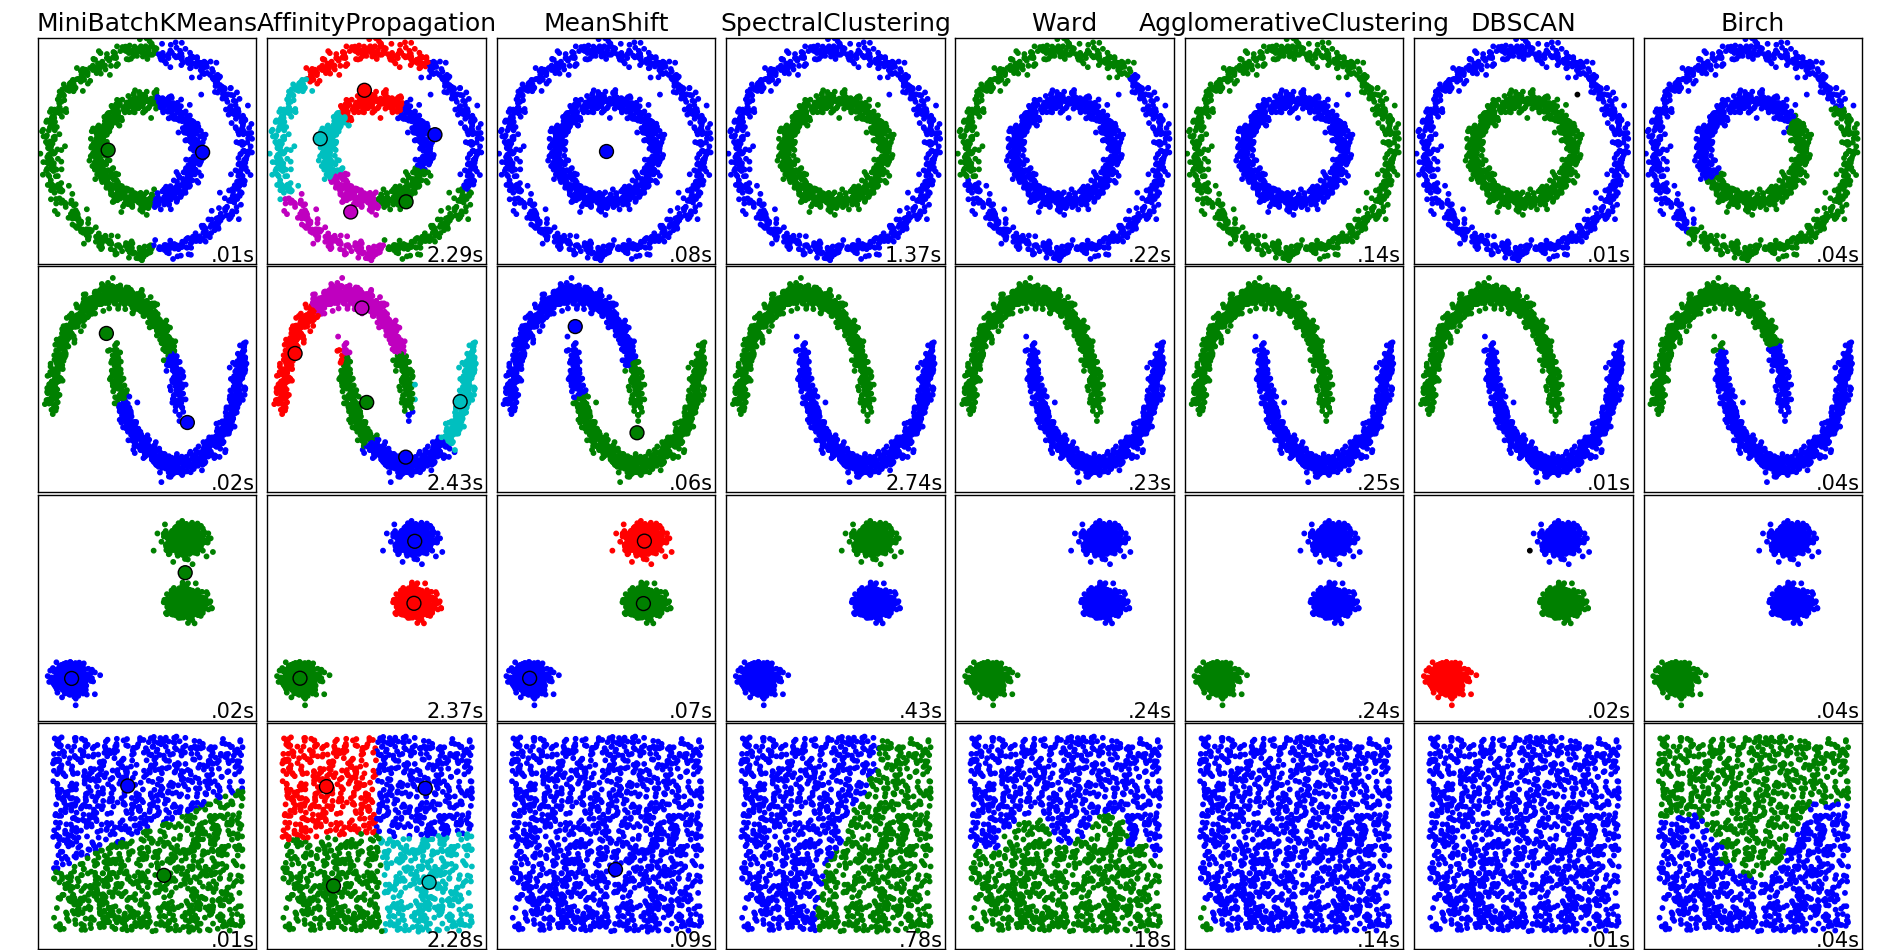
\includegraphics[scale = 0.24]{methods.png}
   \end{center}
   \end{figure}
\end{frame}

\begin{frame}{Самоорганизующаяся карта Кохонена}
	$X$, $\rho:\,X \times X$ --- метрика пространства объектов;

	\vspace{.15cm}
	$Y=\{1,\dots,M\} \times \{1,\dots,H\}$ --- сетка кластеров,\\
	$r: \, Y \times Y$ --- метрика пространства кластеров;

	\vspace{.15cm}
	Каждому узлу $(m,h)$ приписан нейрон Кохонена $w_{mh}\in X$;

	\vspace{.15cm}
	Заданы неотрицательные невозрастающие функции:
	\begin{itemize}
	    \item $K(r(\cdot,\cdot),t)$ --- расстояние,
	    \item $\eta(t)$ --- скорость обучения,
	    \item $\epsilon(t)$ --- окрестность, где $t$ --- номер итерации;
	\end{itemize}

	\vspace{.15cm}
	$\upsilon_{\epsilon(t)}(m_i,h_i)$ --- $\epsilon(t)$-окрестность $(m_i,h_i)$ в метрике $r$:
	\begin{figure}
	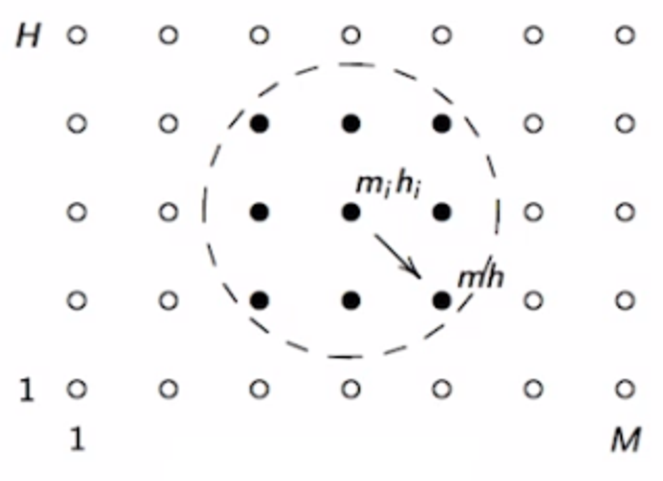
\includegraphics[width=0.4\textwidth]{karta.pdf}
	\end{figure}
\end{frame}

\begin{frame}{Самоорганизующаяся карта Кохонена}
	
	\begin{enumerate}
	\item задать начальные $w_{mh}$, $m=\overline{1:M}$, $h=\overline{1:H}$;
	\item {\bfповторять}
	\item\quad выбрать случайным образом $x_i$ из $X^n$;
	\item\quad вычислить координаты ближайшего кластера:
	$$(m_i,h_i)=\argmin_{(m,h)\in Y}\rho(x_i,w_{mh});$$
	\item\quad {\bfдля всех} $(m,h)\in\upsilon_{\epsilon}(m_i,h_i)$
	\item\qquad сделать шаг стохастического градиентного спуска:\\
	$\qquad w_{mh}=w_{mh}+\eta(t)(x_i-w_{mh})K\left(r[ (m_i,h_i),(m,h) ], t\right);$
	\item {\bfпока} кластеризация не стабилизируется;
	\end{enumerate}
\end{frame}

\begin{frame}{Интерпретация карт Кохонена}
	Два типа графиков -- цветных карт $M\times H$:
	\begin{itemize}
		\item Цвет узла $(m,h)$ --- локальная плотность в точке $(m,h)$ --- среднее расстояние до $k$ ближайших точек выборки;
		\item По одной карте на каждый признак:\\
		цвет узла $(m,h)$ --- значение $j$-й компоненты вектора $w_{mh}.$
	\end{itemize}
	\vspace{.25cm}
	\begin{figure}
		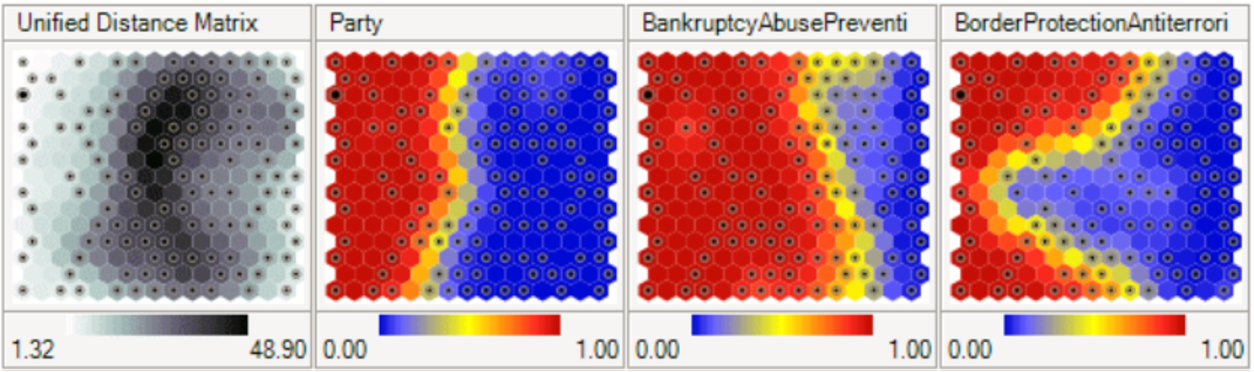
\includegraphics[width=1\linewidth]{koh.pdf}
	\end{figure}
\end{frame}

\begin{frame}{Преимущества и недостатки карт Кохонена}

	\textbf{Преимущества:}
	\begin{itemize}
		\item Возможность визуального анализа многомерных данных.
	\end{itemize}
	\vspace{.5cm}
	\textbf{Недостатки:}
	\begin{itemize}
		\item {\bf Субъективность.} Карта зависит не только от кластерной структуры данных, но и от
		\begin{itemize}
			\item свойств функций $K$, $\eta$, $\epsilon$;
			\item начальных значений $w_{mh}$;
			\item случайного выбора $x_i$ в ходе итераций.
		\end{itemize}
		\item {\bf Искажения.} Близкие объекты исходного пространства могут переходить в далекие точки на карте, и наоборот.
	\end{itemize}
	\vspace{.35cm}
	Рекомендуется только для разведочного анализа данных.
\end{frame}

\begin{frame}{Функционалы качества кластеризации}
   \textbf{Возможна постановка задачи кластеризации:} приписать номера кластеров объектам так, чтобы значение выбранного функционала качества приняло наилучшее значение.\\
   \vspace{4\ex}
   \textbf{Выделяют две группы функционалов качества внутренние и внешние:}
   \begin{itemize}
       \item Среднее внутрикластерное расстояние: $$F_0 = \frac{\sum_{i < j}\mathbf{I}_{\{y_i = y_j\}}\rho(x_i, x_j)}{\sum_{i < j}\mathbf{I}_{\{y_i = y_j\}}},$$
       \item Среднее межкластерное расстояние: $$F_1 = \frac{\sum_{i < j}\mathbf{I}_{\{y_i \neq y_j\}}\rho(x_i, x_j)}{\sum_{i < j}\mathbf{I}_{\{y_i \neq y_j\}}}.$$
   \end{itemize}
   \vspace{4\ex}
   На практике обычно вычисляют $F_0/F_1$.
\end{frame}

\begin{frame}{Функционалы качества кластеризации (Силуэт)}
\begin{itemize}
    \item  Принадлежность объекта своему кластеру:
   \begin{equation*}
    c(x_i) = \frac{1}{|K_i| - 1}\sum\limits_{x_j \in K_i,\, i\neq j}\rho(x_i, x_j)
    \end{equation*}
    \item Принадлежность объекта другому кластеру:
    \begin{equation*}
    b(x_i) = \min\limits_{i\neq j}\frac{1}{|K_j|}\sum\limits_{x_z \in K_j}\rho(x_i, x_z)
    \end{equation*}
    \item  Cилуэт объекта:
    \begin{equation*}
    s(x_i) =
    \begin{cases}
    \frac{b(x_i) - c(x_i)}{\max\{c(x_i), b(x_i)\}}, & |K_i| > 1\\
    0, & |K_i| = 1
    \end{cases}
    \end{equation*}
    \item Cилуэт кластеризации: $S =\frac{1}{n}\sum\limits_{i}s(x_i)$.
\end{itemize}
\vspace{3\ex}
Данный функционал качества пригоден только для кластеров, которые представляют собой далеко отстоящие компактные скопления объектов.
\end{frame}

\begin{frame}{}
   \begin{center}
       \LARGE{Тематические модели}\\
       \vspace{2ex}
       \normalsize{(часть 2)}
   \end{center}
\end{frame}

\begin{frame}{Введение}
   Тематическое моделирование применяется к анализу текстов.
   
   \begin{itemize}
       \item \textit{Тематическое моделирование} --- способ построения модели коллекции текстовых документов. 
       \item Тематическая модель коллекции текстовых документов определяет, к каким темам относится каждый документ и какие слова (термины) образуют каждую тему.
       \item \textit{Вероятностная тематическая модель} описывает каждую тему дискретным распределением на множестве терминов, каждый документ --- дискретным распределением на множестве тем.
   \end{itemize}
\end{frame}

\begin{frame}{Введение}
   Это про выявление тематики в текстовой коллекции...
   \begin{itemize}
       \item  Тема --- условное распределение на множестве терминов $p(w|t)$ --- вероятность термина $w$ в теме $t$;
       \item Тематический профиль документа --- условное распределение $p(t|d)$ --- вероятность темы $t$ в документе $d$.
   \end{itemize}
\end{frame}

\begin{frame}{Задача определения тематики коллекции документов}
\textbf{Дано:}
\begin{itemize}
    \item $W$ --- словарь, множество слов (терминов)
    \item $D$ --- множество (коллекция) текстовых документов
    \item $n_{dw}$ --- частота термина $w \in W$ в документе $d \in D$
\end{itemize}
\vspace{4\ex}
\textbf{Хотим найти:}
\begin{itemize}
    \item число различимых тем\\
    \item какими терминами определяется каждая тема\\
    \item к каким темам относится каждый документ\\
\end{itemize}
или\\
\textbf{Найти:} вероятностную тематическую модель
\end{frame}

\begin{frame}{Гипотезы и допущения}
\begin{itemize}
    \item Гипотеза назвисимости: Порядок слов в документе и порядок документов в коллекции не важны
    \item Гипотеза условной независимости: p(w|d, t) = p(w|t)
    \item Гипотеза разреженности: Каждый документ d и каждый термин w связан с небольшим количеством тем t.
\end{itemize}
\vspace{2\ex}
Если не выполняется гипотеза разреженности?
\begin{itemize}
    \item Документ относится к большому количеству тем $\rightarrow$ разобьем его на части, более однородные по тематике
    \item Термин относится к большому числу тем $\rightarrow$ положим, что термин является общеупотребительным и неважен для определения тематики
\end{itemize}
\end{frame}

\begin{frame}{Вероятностная формализация постановки задачи}
\textbf{Базовые предположения:}\\
каждое слово в документе связано с некоторой темой $t \in T$\\
$D \times W \times T$ --- дискретное вероятностное пространство\\
$D$ --- выборка троек $(d_i, w_i, t_i)^n_{i=1} \sim p(d,w,t)$\\
$d_i,\; w_i$ --- наблюдаемые, $t_i$ --- скрытые (латентные)\\
\vspace{4\ex}
\textbf{Вероятностная модель порождения документа d:}
\begin{equation*}
    p(w, d) = \sum\limits_{t\in T} p(w,d,t) = \sum\limits_{t\in T} p(w|t,d)\cdot p(t,d) =
\end{equation*}
\begin{equation*}
    = \sum\limits_{t\in T} p(w|t,d)\cdot p(t|d) \cdot p(d) = p(d) \cdot \sum\limits_{t\in T} p(w|t)\cdot p(t|d)
\end{equation*}
\vspace{2\ex}
\begin{equation*}
    \fbox{p(w|d) = \sum\limits_{t\in T} p(w|t)\cdot p(t|d)}
\end{equation*}
\vspace{4\ex}
\textbf{Задача:} найти $T,\; p(w|t),\; p(t|d)$.
\end{frame}

\begin{frame}{Предварительная обработка документа}
Необходимость конкретного метода обработки зависит от типа задачи, но вообще это хорошая практика.
\vspace{2\ex}
\begin{itemize}
    \item Лемматизация --- приведение каждого слова в документе к его начальной форме.\\
    \vspace{1\ex}
    \footnotesize Трудоемкий процесс
    \item  \normalsize Стемминг — отбрасывание изменяемых частей слова.\\
    \vspace{1\ex}
    \footnotesize Большое число ошибок
    \item \normalsize Отбрасывание стоп-слов --- удаление слов, которые никак не характеризуют тему.\\
    \vspace{1\ex}
    \footnotesize Почти не влияет на длину словаря
    \item \normalsize Отбрасывание редких слов.\\
    \vspace{1\ex}
    \footnotesize Для коллекций коротких новостных сообщений лучше не использовать
    \item \normalsize Выделение ключевых фраз.\\
    \vspace{1\ex}
    \footnotesize Приходится привлекать экспертов
\end{itemize}
\end{frame}

\begin{frame}{Вероятностная модель порождения документа d}
Вероятностная тематическая модель: $p(w|d) = \sum\limits_{t\in T} p(w|t)\cdot p(t|d)$
\vspace{2\ex}
\begin{figure}
   \begin{center}
   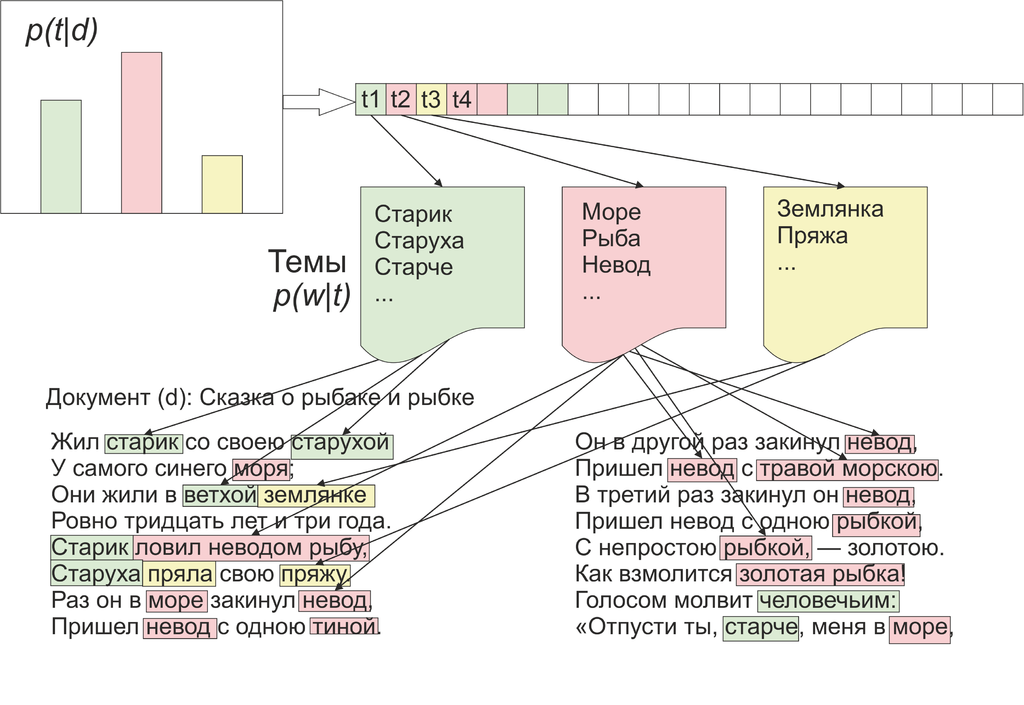
\includegraphics[scale = 1]{Тематическая_модель.png}
   \end{center}
   \end{figure}
\end{frame}

\begin{frame}{Выборочный язык}
\textbf{Дано:} 
\begin{itemize}
    \item коллекция текстовых документов $D$,
    \item $n_{dw}$ --- число вхождений термина $w$ в документ $d$,
    \item $n_d = \sum\limits_{w \in W}n_{dw}$ --- длина документа $d$ в терминах.
\end{itemize}
\vspace{4\ex}
\textbf{Можем оценить:} $\hat{p}(w|d) = \frac{n_{dw}}{n_d}$.\\
\vspace{4\ex}
\textbf{Найти параметры тематической модели:}
\begin{equation*}
    F = \left(\hat{p}(w|d)\right)_{W \times D} \approx \sum\limits_{t \in T}(\varphi_{wt})_{W \times T}(\theta_{td})_{T \times D}
\end{equation*}
\textbf{Искомые:}
\begin{itemize}
    \item $\varphi_{wt} = p(w |t)$ --- вероятности терминов $w$ в каждой теме $t$,
    \item $\theta_{td} = p(t| d)$ --- вероятности тем $t$ в каждом документе $d$.
\end{itemize}
\end{frame}

\begin{frame}{Стохастическое матричное разложение}
Задача стохастического матричного разложения:
\begin{equation*}
    F \approx \Phi\Theta \quad \Leftrightarrow \quad ||F - \Phi\Theta||^{2} \rightarrow  \min\limits_{\Phi,\,\Theta}
\end{equation*}
\begin{figure}
   \begin{center}
   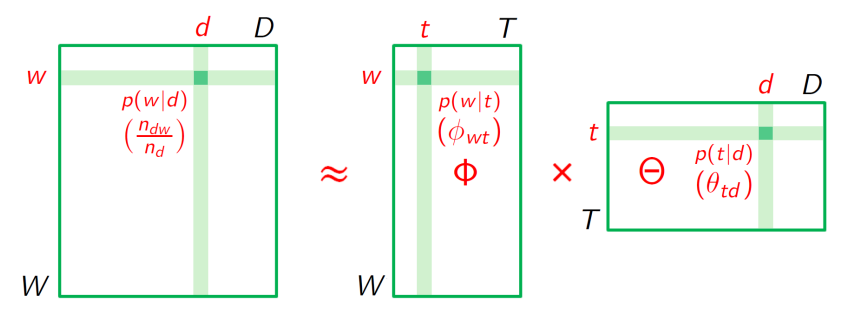
\includegraphics[scale = 0.4]{matrix.png}
   \end{center}
\end{figure}
Если $\Phi$ и $\Theta$ --- решение, то существует матрица $S$ ранга $|T|$: 
\begin{equation*}
    F = \Phi SS^{-1} \Theta,
\end{equation*}
где $S$ --- матрица перестановки, а $\Phi,\, \Theta$ тоже стохастические.
\end{frame}

\begin{frame}{Принцип максимума правдоподобия}
\small
\textbf{Правдоподобие} --- плотность распределения выборки $(d_i, w_i)_{i=1}^n$: 
\begin{equation*}
    \prod\limits_{i=1}^{n}p(d_i, w_i) = \prod\limits_{d \in D}\prod\limits_{w \in W}p(d, w)^{n_{dw}}
\end{equation*}
где $n_{dw}$ --- число вхождений термина $w$ в документ $d$, $n = \sum\limits_{d \in D}\sum\limits_{w \in W}n_{dw}$ --- длина коллекции в терминах.\\
\vspace{4\ex}
\textbf{Максимизация логарифма правдоподобия:}
\begin{equation*}
     \sum\limits_{d \in D}\sum\limits_{w \in W}n_{dw}\ln p(w|d)p(d) \rightarrow \max\limits_{\Phi,\,\Theta},
\end{equation*}
здесь $p(d) = n_d/n = \text{const}$, $n_d$ --- длина документа.\\
\vspace{4\ex}
\textbf{Приходим к задаче:}
\begin{equation*}
     \sum\limits_{d \in D}\sum\limits_{w \in W}n_{dw}\ln \sum\limits_{t \in T}\varphi_{wt}\theta_{td} \rightarrow \max\limits_{\Phi,\,\Theta},
\end{equation*}
При ограничениях неотрицательности и нормировки
\begin{equation*}
     \varphi_{wt} \geq 0; \quad \sum\limits_{w\in W}\varphi_{wt} = 1; \quad \theta_{td}\geq 0; \quad \sum\limits_{t\in T}\theta_{td} = 1.
\end{equation*}
\end{frame}

\begin{frame}{EM-алгоритм}
Для решения задачи матричного разложения применяется \textbf{EM-алгоритм}. Он заключается в выполнении двух шагов до сходимости.\\
\vspace{2\ex}
\textbf{E-шаг:} условные вероятности тем $p(t|d,w)$ для всех $t,\,d,\,w$ вычисляются через $\varphi_{wt},\, \theta_{td}$ по формуле Байеса:
\begin{equation*}
    H_{dwt} = p(t| d, w) = \frac{p(w,t |d)}{p(w | d)} = \frac{p(w |t)p(t| d)}{p(w | d)} = \frac{\varphi_{wt}\theta_{td}}{\sum\limits_{s\in T}\varphi_{ws}\theta_{sd}}. 
\end{equation*}
\vspace{2\ex}
\textbf{M-шаг:} частотные оценки условных вероятностей вычисляются путем накопления счетчика $n_{dwt} = n_{dw}p(t|d,w)$:
\begin{equation*}
    \varphi_{wt} = \frac{\hat{n}_{wt}}{\hat{n}_{t}},\quad \hat{n}_t =\sum\limits_{w \in W}\hat{n}_{wt},\quad \hat{n}_{wt} = \sum\limits_{d \in D}n_{dw}H_{dwt};
\end{equation*}
\begin{equation*}
     \theta_{dt} = \frac{\hat{n}_{dt}}{\hat{n}_{t}},\quad \hat{n}_d =\sum\limits_{t \in T}\hat{n}_{dt},\quad \hat{n}_{dt} = \sum\limits_{w \in W}n_{dw}H_{dwt}.
\end{equation*}
\end{frame}

\begin{frame}{Модификация EM-алгоритма}
Можно не хранить матрицу $H_{dwt}$ и уменьшить вычислительные затраты, получим алгоритм:\\
\begin{figure}
   \begin{center}
   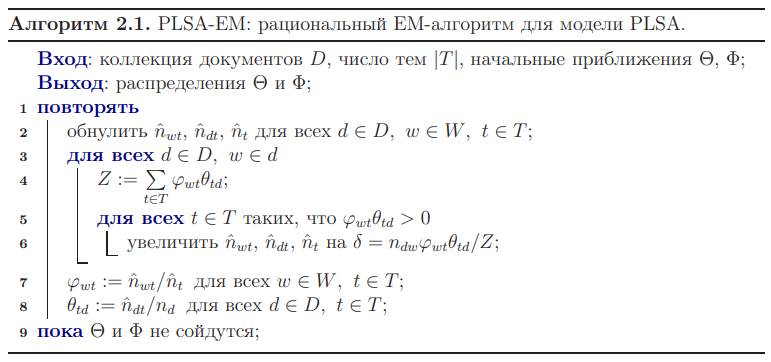
\includegraphics[scale = 0.55]{Em-алг.png}
   \end{center}
\end{figure}
\end{frame}

\begin{frame}{Начальное приближение $\varphi_t$, $\theta_d$}
\footnotesize
\begin{enumerate}
    \item Начальное приближение можно задать нормированными случайными векторами из равномерного распределения.
    \item Пройти по всей коллекции, выбрать для каждой пары $(d, w)$ случайную тему $t$, вычислить частотные оценки вероятностей $\varphi_{wt}$ и $\theta_{td}$ для всех $d,\, w,\, t$.
    \item \textbf{Частичное обучение} (некоторые $t$ известны заранее и имеются дополнительные данные о привязке некоторых $d$ или $w$ к $t$):
    
    Известно, что документ $d$ относится к подмножеству $T_d \subset T$:
        \begin{equation*}
        \theta_{td}^{0} = \frac{1}{|T_d|}\mathbf{I}_{t \in T_d}.
        \end{equation*}
    Известно, что подмножество терминов $W_t \subset W$ относится к теме t:
        \begin{equation*}
        \varphi_{wt}^{0} = \frac{1}{|W_t|}\mathbf{I}_{w \in W_t}.
        \end{equation*}
    Известно, что некоторое множество документов $D_t \subset D$ относится к теме $t$:
        \begin{equation*}
        \varphi_{wt}^{0} = \frac{\sum_{d \in D_t}n_{dw}}{\sum_{d \in D_t}n_{d}}.
        \end{equation*}
    
\end{enumerate}
\end{frame}

\begin{frame}{Недостатки PLSA}
\begin{itemize}
    \item Задача стохастического матричного разложения некорректно поставлена (может быть бесконечно много решений), это приводит к неустойчивости матриц $\Phi$ и $\Theta$;
    \vspace{2\ex}
    \item С появлением нового d не можем вычислить p(t|d), не перестраивая модель;
    \vspace{2\ex}
    \item Число параметров растёт линейно по числу документов в коллекции, что может приводить к переобучению модели.
\end{itemize}
\end{frame}

\begin{frame}{Внутренние (intrinsic) критерии качества тематической модели}
\textbf{Перплексия} (perplexity) языковой модели $p(w|d)$:
\begin{equation*}
    \mathcal{P}(D) = \exp \left( -\frac{1}{n}\sum\limits_{d \in D}\sum\limits_{w \in d}n_{dw}\ln p(w|d)\right), \; n = \sum\limits_{d \in D}\sum\limits_{w \in d}n_{dw}.
\end{equation*}
\vspace{4\ex}
\textbf{Интерпретация:}
\begin{itemize}
    \item если $p(w|d) = \frac{1}{|W|}$, то $\mathcal{P} = |W|$;
    \item мера неопределенности в тексте.
\end{itemize}
\end{frame}

\begin{frame}{Перплексия тестовой коллекции}
Перплексия тестовой коллекции $D^{'}$ (hold-out perplexity):
\begin{equation*}
    \mathcal{P}(D^{'}) = \exp \left( -\frac{1}{n^{''}}\sum\limits_{d \in D^{'}}\sum\limits_{w \in d^{''}}n_{dw}\ln p(w|d)\right), \; n^{''} = \sum\limits_{d \in D^{'}}\sum\limits_{w \in d^{''}}n_{dw}.
\end{equation*}
\vspace{2\ex}
$d = d^{'} \cup d^{''}$ --- случайное разбиение тестового документа на две половины равной длины;
\vspace{2\ex}
\begin{itemize}
    \item параметры $\varphi_{wt}$ оцениваются по обучающей коллекции $D$
    \item параметры $\theta_{td}$ оцениваются по первой половине $d^{'}$
    \item перплексия вычисляется по $d^{''}$
\end{itemize}
\end{frame}

\begin{frame}{Когерентность как мера интерпретируемости}
Когерентность (согласованность) темы $t$ по $k$ топовым словам:
\begin{equation*}
    \text{PMI}_{t} = \frac{2}{k(k-1)}\sum\limits_{i=1}^{k-1}\sum\limits_{j =i+1}^{k}\text{PMI}(w_i, w_j),
\end{equation*}
где $w_i$ --- $i$-й термин в порядке убывания $\varphi_{wt}$.\\
\vspace{2\ex}
$\text{PMI}(u, v) = \ln{\frac{|D|N_{uv}}{N_uN_v}}$ --- поточечная взаимная информация (pointwise mutual information),\\
\vspace{2\ex}
$N_{uv}$ --- число документов, в которых термины $u,\, v$ встречаются рядом,\\
\vspace{2\ex}
$N_{u}$ --- число документов, в которых $u$ встретился хотя бы раз.
\end{frame}

\end{document}